\documentclass{styles/my_class}         % Clase personalizada 
\usepackage{styles/custom-style}     % Cargar el estilo desde 'config/mi_estilo.sty'
 
%=== Glosario===
 % Glosario personalizado
 \newglossary[glgcon]{constantes}{glscon}{glocon}{Glosario Definido por el usuario}%(/tex/03-Referencia_Configuracion/02-definicion_glosarios)
 %======================================================================
% === Glosario de términos generales (type: main) ===
%======================================================================
\newglossaryentry{algoritmo}{
  name={\textbf{alg}},
  plural={\textbf{algs}},
  description={conjunto de pasos definidos para resolver un problema}
}

\newglossaryentry{modelo}{
  name={\textbf{modelo}},
  plural={\textbf{modelos}},
  description={representación simplificada de un sistema o fenómeno}
}
%======================================================================
% === Glosario de acrónimos y siglas (type: acronym) ===
%======================================================================
\newacronym[longplural={Unidades Centrales de Procesamiento}]{cpu}{\textbf{CPU}}{Unidad Central de Procesamiento}
\newacronym[longplural={Unidades de Procesamiento Gráfico}]{gpu}{\textbf{GPU}}{Unidad de Procesamiento Gráfico}
%======================================================================
% === Glosario de símbolos (type: symbols) ===
%======================================================================
\newglossaryentry{alpha}{
  type=symbols,         
  name={\textbf{$\alpha$}},
  description={coeficiente de expansión térmica}
}

\newglossaryentry{lambda}{ 
  type=symbols,
  name={\textbf{$\lambda$}},
  description={longitud de onda}
}

%======================================================================
% === Definido por el usuario ===
%======================================================================
\newglossaryentry{planck}{
  type=constantes,
  name={\textbf{$h$}},
  description={constante de Planck: \(6.626 \times 10^{-34}~\text{J$\cdot$s}\)}
}

\newglossaryentry{gravitacional}{
  type=constantes,
  name={\textbf{$G$}},
  description={constante de gravitación universal: $6.674 \times 10^{-11}~\text{N·m}^2/\text{kg}^2$}
}
  % Carga las definiciones de glosario
 \makeglossaries

%=== Bibliografia===
 \addbibresource{tex/03-Referencia_Configuracion/01-references.bib} % (/tex/03-Referencia_Configuracion/01-references.bib)


\begin{document}
%=============================================================
% Partes preliminares
%=============================================================
 \begingroup 
 \let\cleardoublepage\clearpage % No genera hoja al terminar impar
 \thispagestyle{empty}
 
\begin{titlepage}
  \thispagestyle{empty} % Sin numeración de página
  \AddToShipoutPictureBG*{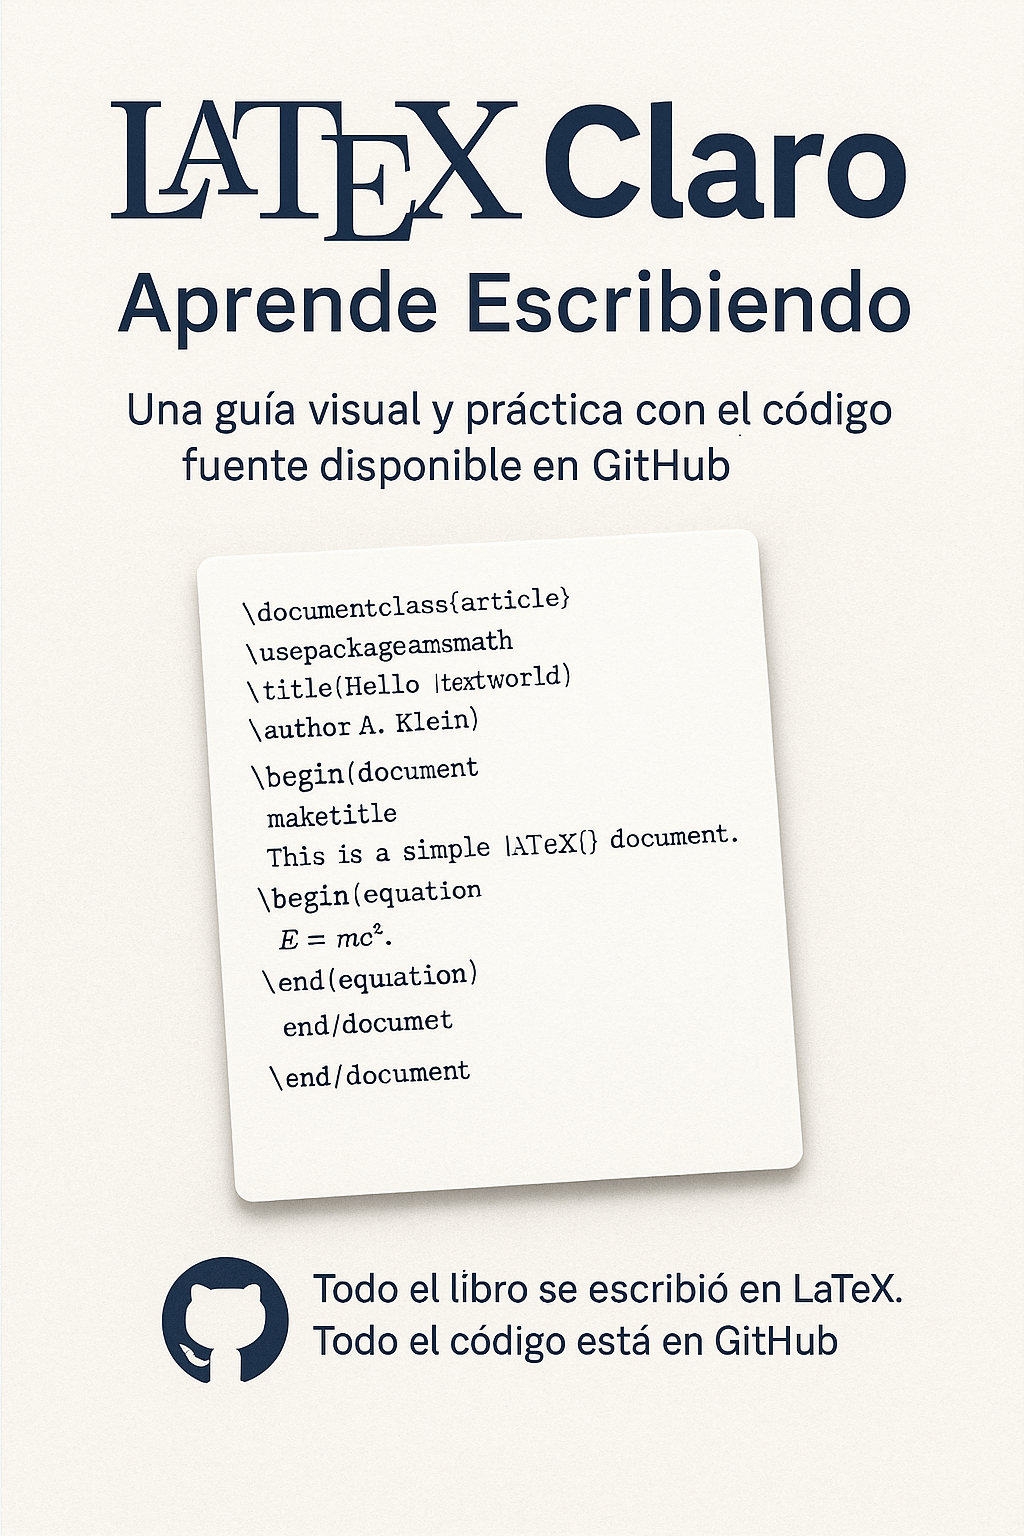
\includegraphics[width=\paperwidth,height=\paperheight]{images/tex.png}}%
  \vspace*{\fill} % Para evitar solapamientos

\end{titlepage}

 \clearpage
 \addcontentsline{toc}{chapter}{Acerca de la obra}

\clearpage

\begin{titlepage}
    \thispagestyle{empty} % Sin numeración de página
    \vfill

    
    \begin{center}
        
        \vspace*{2cm}
        \textcolor{black}{\Huge \textbf{Plantilla de Libro}} \\[0.7cm] % Título
        {\large Primera Edición} \\[0.3cm]  % Subtítulo

        % Línea decorativa
        \rule{\textwidth}{0.4pt} \\[1cm]

        {\Huge \textit{Yael R.G.}} \\[0.5cm]  % Autor 1
        {\normalsize Lic. M.A.C.} \\[1.5cm]  % Títulos Autor 1

        {\Huge \textit{Autor 2}} \\[0.5cm]  % Autor 2
        {\normalsize Títulos del Autor 2} \\[8cm]  % Títulos Autor 2
        \maketitle

        % Logotipo
        
\includegraphics[width=3cm]{images/y.png} \\[1cm]  % Logotipo

        % Información de la editorial
        {\Large Editorial: Autopublicado} \\[1cm]  % Editorial
        {\large C.D.M.X, 2025}  % Ciudad y año de publicación
            
    \end{center}
    \vfill
\end{titlepage}
\clearpage
 \clearpage
 
\thispagestyle{empty} % Sin numeración en esta página

\begin{center}
\vspace*{1cm}
\textcolor{black}{\Large \textbf{© 2025, Yael R.G.}} \\[0.3cm]


Plantilla creada por Yael R.G. \\[0.3cm]
Créditos: \url{https://www.linkedin.com/in/yael-rg-digital}. \\[0.3cm]
Disponible en: \url{https://github.com/YaelRosas/professional-latex-book-template} \\[0.5cm]

\textbf{Licencia:} Creative Commons Attribution 4.0 International License (CC BY 4.0). \\[0.5cm]

\begin{center}
    Puede encontrar un resumen de la licencia en: \\
    \url{https://creativecommons.org/licenses/by/4.0/} \\[0.5cm]
    
    El código legal completo está disponible en: \\
    \url{https://creativecommons.org/licenses/by/4.0/legalcode}
    \end{center}
    

\textbf{Usted es libre de:}
\end{center}

\begin{center}
\begin{tabular}{c}
    \begin{minipage}{0.9\textwidth}
    \color{black}
    \begin{itemize}
        \item \textbf{Compartir} — copiar y redistribuir el material en cualquier medio o formato.
        \item \textbf{Adaptar} — remezclar, transformar y construir sobre el material para cualquier propósito, incluso comercialmente.
    \end{itemize}
    \end{minipage}
    \end{tabular}    
\end{center}

\begin{center}
\textbf{Bajo los siguientes términos:}
\end{center}

\begin{center}
\begin{tabular}{c}
\begin{minipage}{0.9\textwidth}
\color{black}
\begin{itemize}
    \item \textbf{Atribución} — Debe dar el crédito apropiado, proporcionar un enlace a la licencia e indicar si se han realizado cambios. Puede hacerlo de cualquier manera razonable, pero no de ninguna manera que sugiera que el licenciante lo respalda a usted o a su uso.
    \item \textbf{Sin restricciones adicionales} — No puede aplicar términos legales o medidas tecnológicas que restrinjan legalmente a otros a hacer cualquier cosa que permita la licencia.
\end{itemize}
\end{minipage}
\end{tabular}
\end{center}

\begin{center}
{\large Primera edición, 2025} \\[0.5cm]

{\large \textbf{Equipo de Edición:}} \\[0.5cm]
{\large Editor: Yael RG} \\[0.5cm]
{\large Técnico editorial: ChatGPT (OpenAI)} \\[1.0cm]

{\large \textbf{Equipo de Diseño:}} \\[0.5cm]
{\large Diseñador: Yael RG} \\[0.5cm]
{\large Técnico de diseño: ChatGPT (OpenAI)} \\[1.0cm]
\end{center}


 \endgroup
 
 \frontmatter % Inicia numeración romana
 
\thispagestyle{empty} % Sin numeración en esta página

\begin{center}
    \vspace*{2cm}

    % Ejemplos 
    {\Huge \textbf{Dedicatoria}} \\[1.5cm]
    
    {\large A familia, por su comprensión y paciencia durante este proceso.} \\[1.5cm]
    
    \vspace*{3cm}
    {\large \textbf{Nombre del Autor}} \\[1.0cm]
    {\large Ciudad, Año}

\end{center}

\vfill
\clearpage
 
 
\thispagestyle{empty} % Sin numeración de página


\vspace*{2cm}

% Ejemplos 
{\Huge \textbf{Agradecimientos}} \\[1.0cm]
 

Quiero expresar mi más sincero agradecimiento a todas las personas que contribuyeron a la creación de esta obra. En particular:

\begin{center}
\begin{itemize}
    \item A \textbf{[Mentor, experto]}, por sus valiosos comentarios durante el desarrollo de este proyecto.
    \item A \textbf{[Equipo o colaboradores]}, cuyo trabajo fue esencial para completar este libro.
    \item A mi familia y amigos, por su paciencia, comprensión y aliento.
\end{itemize}
\end{center}
A todos ustedes, gracias por hacer que este proyecto sea una realidad.
\clearpage 
 
\vspace*{2cm}

% Ejemplos 
{\Huge \textbf{Epigrafe}} \\[1.0cm]
 

% Puedes incluir múltiples epígrafes si lo necesitas:

\epigraph{
    ``La inteligencia no es la capacidad de almacenar información, sino de saber dónde encontrarla.''
}{
    -- Albert Einstein
}

\vspace{2cm} % Espaciado opcional entre epígrafes
\epigraph{
    ``El éxito consiste en ir de fracaso en fracaso sin perder el entusiasmo.''
}{
    -- Winston Churchill
}

\clearpage
 \thispagestyle{empty}
\vspace*{2cm}

% Ejemplos 
{\Huge \textbf{Prólogo}} \\[1.0cm]
 
Introducciòn que ofrece una visión general del contenido.

\textbf{Estructura sugerida para el prólogo:}
\begin{enumerate}
    \item **Introducción**: Presentar brevemente el libro y su importancia.
    \item **Contexto**: Explicar cómo el libro encaja en el campo o área del conocimiento.
    \item **Recomendación**: Resaltar por qué el lector debería continuar leyendo el libro.
    \item **Firma del autor del prólogo**: Agregar el nombre, título o cargo de la persona que lo escribe.
\end{enumerate}

 
\vspace{2em}
\hfill \textit{[Nombre del autor del prólogo]} \\
\hfill \textit{[Título o cargo]} \\
\hfill \textit{[Lugar y fecha]} \\
\clearpage
 \thispagestyle{empty}
\vspace*{2cm}
\textcolor{black}{\Huge \textbf{Prefacio}} \\[0.7cm] % Título
El prefacio, escrito por el autor principal del libro, ofrece una visión general de las motivaciones
detrás de la obra, el enfoque adoptado, los objetivos perseguidos y la audiencia a la que está dirigida.

\vspace*{2cm}
\textbf{Ejemplo:}

Este libro nace de mi deseo de compartir el conocimiento adquirido en el campo de ... , 
con el objetivo de crear un recurso integral para principiantes y expertos. 
 Espero que esta obra sirva como herramienta útil para quienes deseen explorar y desarrollar soluciones innovadoras.
 
 \vspace*{2cm}
--- *Nombre del autor*  
\clearpage
 \thispagestyle{empty}
\vspace*{2cm}
\textcolor{black}{\Huge \textbf{Tabla de Contribuciones}} \\[0.7cm] % Título

Esta tabla presenta a los contribuyentes que han colaborado en la creación de este libro,
detallando sus roles y las áreas específicas en las que han brindado su apoyo.

\begin{itemize}
    \item \textbf{Prólogo:}  
    El prólogo ha sido escrito por la Dra. ... , profesora e investigadora en .... .
    
    \item \textbf{Capítulo X:}  
    El capítulo sobre ... fue revisado y ampliado por el Ing. ...., especialista en .... 

    \item \textbf{Revisión Técnica:}  
    La revisión técnica del manuscrito fue realizada por la organización ...., asegurando precisión y claridad en los conceptos presentados.

    \item \textbf{Edición y Formato:}  
    Agradecemos a Editorial ... por su trabajo excepcional en la edición y formato final del documento.
\end{itemize}
\clearpage
 \thispagestyle{empty}
\vspace*{2cm}
\textcolor{black}{\Huge \textbf{Nota del autor}} \\[0.7cm] % Título

Se destacan aclaraciones, comentarios adicionales, reflexiones sobre el contenido del libro, 
o detalles importantes para una mejor comprensión del texto.

Este libro fue escrito con la intención de compartir conocimientos adquiridos ....\\

Pretende ser un punto de partida.\\

Las opiniones expresadas aquí son personales y no representan necesariamente la postura de ninguna institución.
\clearpage
 \clearpage
 \tableofcontents

\let\cleardoublepage\clearpage % Evita página en blanco tras páginas impares

\renewcommand{\listfigurename}{Lista de Figuras}
\clearpage
\thispagestyle{empty} % Oculta número en esta página
\listoffigures

\renewcommand{\listtablename}{Lista de Tablas}
\clearpage
\thispagestyle{empty}
\listoftables
\clearpage
%=============================================================
% Cuerpo del libro
%=============================================================
 \mainmatter % Inicia numeración arábiga
 \cleardoublepage
\chapter*{Introducción}
\addcontentsline{toc}{chapter}{Introducción}  % Añadir al índice manualmente

% 11-introduction.tex

La introducción de tu libro o proyecto debe proporcionar una visión general de los temas que se tratarán, los objetivos del proyecto y cualquier otra información relevante. 

En esta sección puedes incluir:

\begin{itemize}
    \item El propósito del libro o proyecto.
    \item Breve descripción de los temas que se abordarán.
    \item Objetivos y metas principales.
    \item Información relevante para el lector.
\end{itemize}

Puedes agregar más detalles y personalizar esta plantilla según sea necesario para tu proyecto.
 
 \pagenumbering{arabic} % Evita duplicados en numeración
\cleardoublepage

% ============================
% SECCIÓN: ESTRUCTURA GENERAL DE UN CAPÍTULO 
 %(sección 6 en config.tex)
%=================
\chapter{Capitulo}
\fancyhead{} % Borra el encabezado
\thispagestyle{fancy}

Texto...Texto...Texto...Texto...Texto...Texto...Texto...Texto...Texto...

Texto...Texto...Texto...Texto...Texto...Texto...Texto...Texto...Texto...
\section{Seccion} 
Texto...Texto...Texto...Texto...Texto...Texto...Texto...Texto...Texto...

Texto...Texto...Texto...Texto...Texto...Texto...Texto...Texto...Texto...
\subsection{Subseccion}
Texto...Texto...Texto...Texto...Texto...Texto...Texto...Texto...Texto...

Texto...Texto...Texto...Texto...Texto...Texto...Texto...Texto...Texto...
\subsubsection{Subsubsection}

\paragraph{Parrafo}
Texto...Texto...Texto...Texto...Texto...Texto...Texto...Texto...Texto...

Texto...Texto...Texto...Texto...Texto...Texto...Texto...Texto...Texto...
\subparagraph{Subparrafo}
Texto...Texto...Texto...Texto...Texto...Texto...Texto...Texto...Texto...

Texto...Texto...Texto...Texto...Texto...Texto...Texto...Texto...Texto...


 % ======== 
 % Solution
 \begin{activity}[Trabaja en parejas]
  Encuentra tres ejemplos de grupos que no sean abelianos.
\end{activity}

\begin{definition}[Este término es clave]
  Un \emph{grupo} es un conjunto con una operación binaria que satisface la asociatividad, tiene un elemento neutro y cada elemento posee un inverso.
\end{definition}

\begin{example}[Grupo simple]
  El conjunto de los enteros \( \mathbb{Z} \) con la suma es un grupo.
\end{example}

\begin{exercise}[Intenta resolverlo]
  Demuestra que el conjunto de los enteros pares forma un subgrupo de \( \mathbb{Z} \).
\end{exercise}

\begin{generality}[Por qué importa la generalidad]
  El concepto de grupo abstrae la idea de simetría, aplicable en álgebra, geometría y física.
\end{generality}

\begin{note}[Consejo sobre notación]
  El elemento neutro suele denotarse por \( e \) o \( 1 \), según el contexto.
\end{note}

\begin{property}[Clausura]
  El producto de dos elementos cualesquiera de un grupo pertenece también al grupo.
\end{property}

\begin{remark}[Confusión común]
  Recuerda: la operación del grupo no tiene que ser multiplicación.
\end{remark}

\begin{solution}[prueba de conteo]
  La derivada de \( f(x) = x^2 \) es \( f'(x) = 2x \).
  Aplicamos la regla de la potencia para obtener este resultado.
\end{solution}

\begin{summary}[Ideas clave del capítulo]
  Este capítulo abordó la definición formal de grupo, ejemplos importantes como \((\mathbb{Z}, +)\), y propiedades clave como la existencia del neutro e inverso.
\end{summary}

\begin{theorem}[Propiedad básica de los grupos]
  Si \( G \) es un grupo y \( a, b \in G \), entonces \( ab^{-1} \in G \).
\end{theorem}

\begin{warnbox}[Precaución al usar propiedades conmutativas]
  No todas las operaciones son conmutativas. Asegúrate de verificar las propiedades antes de aplicarlas.
\end{warnbox}
    
%===========================================================
 \section{Entornos predefinidos} 
 
  quote	      Sangrado especial
  quotation	  Similar a quote
  verse	      Para poesía (maneja saltos de línea)
  center	    Centra texto
  flushleft	  Alinea a la izquierda
  flushright	Alinea a la derecha
  itemize	    Lista con viñetas
  enumerate	  Lista numerada
  description	Lista con etiquetas personalizadas
 

\section{Jerarquía de secciones}

Los comandos de jerarquía de secciones son utiles para generar el índice y agregar "títulos". 

\begin{center}
  \begin{tabular}{|c|l|c|}
  \hline
  \textbf{Nivel} & \textbf{Etiqueta} & \textbf{Disponible en} \\
  \hline
  0 & \verb|\part| & \verb|book| o \verb|report| \\
  1 & \verb|\chapter| & \verb|book| o \verb|report| \\
  2 & \verb|\section| & Todas las clases \\
  3 & \verb|\subsection| & Todas las clases \\
  4 & \verb|\subsubsection| & Todas las clases \\
  5 & \verb|\paragraph| & Todas las clases \\
  6 & \verb|\subparagraph| & Todas las clases \\
  \hline
  \end{tabular}
  \end{center}

Sin embargo, \textbf{no están pensadas para ser usadas como simples contenedores de texto}.  
Si se desea escribir párrafos de texto normales, lo correcto es usar líneas en blanco entre bloques de texto en vez de estas.

\begin{custompar}
  Si se desea escribir párrafos con formato personalizado, lo recomendable es definir un entorno personalizado usando 
  \textbf{\texttt{\textbackslash newenvironment}} en el archivo de configuración (sección 6 en este proyecto,tambien se puede modificar el formato del texto general).
  \end{custompar}

% ============================
%  Alineaciones de párrafos: 
 
 \textbf{Alineaciones de párrafos}

 \begin{flushleft}
 Este párrafo estará alineado a la izquierda.
 \end{flushleft}
 
 \begin{center}
 Este párrafo estará centrado.
 \end{center}
 
 \begin{flushright}
 Este párrafo estará alineado a la derecha.
 \end{flushright}
 
% ============================
%  Texto con marcos 
 
\textbf{Texto con marcos}
 
 % Requiere: \usepackage{framed}
 \begin{framed}
 Este párrafo está dentro de un marco.
 \end{framed}
 
 % Requiere: \usepackage{mdframed}
 \begin{mdframed}
 Este párrafo está dentro de un marco con más opciones de estilo.
 \end{mdframed}
 
 \clearpage
% ============================
% SECCIÓN: EJEMPLO LISTAS
 %(seccion 14 en config.tex)
 
 \section{Ejemplo de listas}
 
  \subsection{Lista estandar}
   Ejemplo \texttt{Titulo de la lista}:


  
  \subsection{Lista con titulos definidos}
   \begin{description}
      \item[Contexto:] Comprender el contexto histórico del tema.
      \item[Problema:] Identificar los problemas clave a resolver.
      \item[Revisión:] Revisar trabajos previos relevantes.
    \end{description}
    
    \clearpage
% ============================
% SECCIÓN: EJEMPLO DE CITAS Y BIBLIOGRAFIA
 % (seccion 12 en config.tex)
 % Requisitos (ya estan implementados):
 %  
 % 1-Cargar el archivo .bib en  main.tex (Justo despues de \documentclass) 
 % 2-Definir la cita en el archivo .bib (En /tex/Material_de_referencia)
 % 3-Imprimir la bibliografia con \printbibliography (Esta al final del main.tex)
 \section{Ejemplo de citas}
 
 % Cómo citar en LaTeX (bibliografía .bib)

 Este es un ejemplo de cita de un libro: \cite{EjemploLibro}.  
 Se usa para referirse a libros, artículos, documentación, etc.
 
 % Archivo .bib obligatorio
 Las citas deben estar definidas en un archivo \textbf{bib.}  
 En este proyecto
 
 % Mostrar bibliografía al final
 El comando \texttt{\textbf{printbibliography}} imprime solo las fuentes citadas en el documento.  
Se coloca normalmente en las últimas partes del documento, como en \texttt{\textbf{main.tex}}.

El comando \texttt{\textbf{nocite\{*\}}} fuerza a incluir todas las entradas del archivo \texttt{\textbf{.bib}}, incluso si no fueron citadas.
 % Ejemplo de cita textual corta
 \begin{quote}
 Esta es una cita corta. Se muestra con márgenes más estrechos.
 \end{quote}
 
 % Ejemplo de cita textual larga
 \begin{quotation}
 Esta es una cita más larga.
 
 Puede contener varios párrafos.
 \end{quotation}
 \clearpage
% ============================
%  SECCIÓN: EJEMPLO NOTAS AL PIE Y REFERENCIAS
 %(seccion 12 en config.tex)
 
 \section{Ejemplo de notas al pie de página y referencias cruzadas}

 Este ejemplo muestra cómo crear referencias cruzadas y notas al pie de página en \LaTeX.
 
 Para crear una referencia cruzada, utiliza el comando \textbf{\texttt{\textbackslash label\{etiqueta\}}}
 para asignar una etiqueta a una sección. Luego, usa \textbf{\texttt{\textbackslash ref\{etiqueta\}}} o 
 \textbf{\texttt{\textbackslash autoref\{etiqueta\}}} para referenciarla en otra parte del documento.
 
 Para agregar una nota al pie, utiliza \textbf{\texttt{\textbackslash footnote\{texto de la nota\}}}.
 
 

\footnote{Coloca el comando justo donde deseas que aparezca el número de la nota al pie.}
 
 \subsection{Sección de ejemplo} 

 \label{sec:ejemplo}% Lleva a lo que este abajo de la etiqueta
 Esta sección de ejemplo es referenciada con \texttt{\textbackslash label\{etiqueta\}}.


 Texto...Texto...Texto...Texto...Texto...Texto...Texto...Texto...Texto...

 Texto...Texto...Texto...Texto...Texto...Texto...Texto...Texto...Texto...

 Texto...Texto...Texto...Texto...Texto...Texto...Texto...Texto...Texto...

 Referencia al apendice A \autoref{sec:Apendice A}

 \subsection{Referencia cruzada} 
 Para más información, consulta la \autoref{sec:ejemplo}, que contiene detalles sobre cómo usar notas al pie 
 y referencias cruzadas.
 En esta parte vamos a poner la nota a pie de pagina\footnote{Ejemplo nota al pie de pagina}
 
 las notas tambien pueden tener referencias\footnote{\autoref{sec:ejemplo}}

 \clearpage 
% ============================
%  SECCIÓN: EJEMPLO GLOSARIOS, ABREVIACIONES, SIGLAS Y SIMBOLOS 
 %  (sección 11 en config.tex)
 %  Las entradas se cargan desde un archivo externo (17-glossary.tex)
 %  Se incluye en main.tex con: 
 %     \input{tex/03-Material_de_referencia/17-glossary.tex}
 
 \section{Ejemplo de uso de glosarios definidos}

 \textbf{Los glosarios se imprimen al final del documento*}
 Después de la primera mención de un acrónimo,
 las siguientes veces que uses la misma etiqueta mostrará la forma abreviada. 
 % ============================
 \subsection{Glosario de términos generales}
 
 % Las entradas definidas con \newglossaryentry sin "type=" van al glosario principal.
 
 En este caso la abreviacion siempre se muestra corta:
 algoritmo abreviacion = \gls{algoritmo} 
 si se define se puede usar una forma plural =  \glspl{algoritmo}  
 otro  ejemplo mal definido = \gls{modelo} 
 
 % ============================
 \subsection{Lista de abreviaciones y siglas}
 
 Las siglas definidas con newacronym se imprimen completas la primera vez, luego abreviadas.
 
 La \gls{cpu} realiza las tareas básicas de procesamiento.  
 Una \gls{gpu} moderna puede acelerar algoritmos complejos.
 Por su parte, la \gls{gpu} es más eficiente para el procesamiento gráfico intensivo.  
 
 % ============================
 \subsection{Glosario de símbolos}
  
 % Entradas definidas con type=symbols. El nombre puede tener notación matemática.
 Para usar  un glosario personalizado hay que definir el glosario en el preambulo de tu main 

 El símbolo \gls{alpha} representa el coeficiente de expansión térmica.  
 La \gls{lambda} indica la longitud de onda en fenómenos ondulatorios.
 
 \subsection{Ejemplo de uso de glosarios personalizados}
 
 La constante de Planck, representada por \gls{planck}, es fundamental en la teoría cuántica.  
 La constante de gravitación universal, denotada por \gls{gravitacional}, juega un papel crucial en la física gravitacional.

 \clearpage 
% ============================
%  SECCIÓN: EJEMPLO FIGURAS Y TABLAS
 %(seccion 9 en config.tex)

 \clearpage % Fuerza salto de página para procesar cualquier figura/tabla pendiente
 \section{Figuras y tablas}

 Este capítulo ofrece ejemplos prácticos de cómo trabajar con tablas y figuras en \LaTeX.
 
 % ----------------------------
 % SUBSECCIÓN: TABLAS
 % ----------------------------
  
  \subsection{Tablas en \LaTeX}
  
  \begin{table}[H] % [H] del paquete float obliga a poner la tabla exactamente aquí
      \centering
      \begin{tabular}{|c|c|c|} % Tres columnas centradas con bordes verticales
          \hline
          \textbf{ID} & \textbf{Nombre} & \textbf{Edad} \\
          \hline
          1 & Juan Pérez  & 30 \\
          2 & María López & 25 \\
          3 & Luis García & 35 \\
          \hline
      \end{tabular}
      \caption{Ejemplo de tabla creada con \LaTeX.}
      \label{tab:ejemplo_tabla}
  \end{table}
  
 % Usando booktabs
 \subsubsection{Usando booktabs}

 \begin{table}[H]
   \centering
   \begin{tabular}{ccc}
     \toprule
     ID & Nombre & Edad \\
     \midrule
     1 & Juan Pérez  & 30 \\
     2 & María López & 25 \\
     3 & Luis García & 35 \\
     \bottomrule
   \end{tabular}
   \caption{Tabla con estilo \texttt{booktabs}.}
   \label{tab:booktabs}
 \end{table}
 
  \subsubsection{Consejos sobre tablas}
  Si las tablas son simples, se pueden escribir directamente como en el ejemplo anterior.  
  Para tablas extensas que ocupen varias páginas, se recomienda usar el paquete `longtable` o `tabu`.
 
 % ----------------------------
 % SUBSECCIÓN: FIGURAS
 % ----------------------------
  
  \subsection{Figuras en \LaTeX}
  
  Ejemplo de cómo insertar imágenes externas:
  
  \begin{figure}[H]
      \centering
      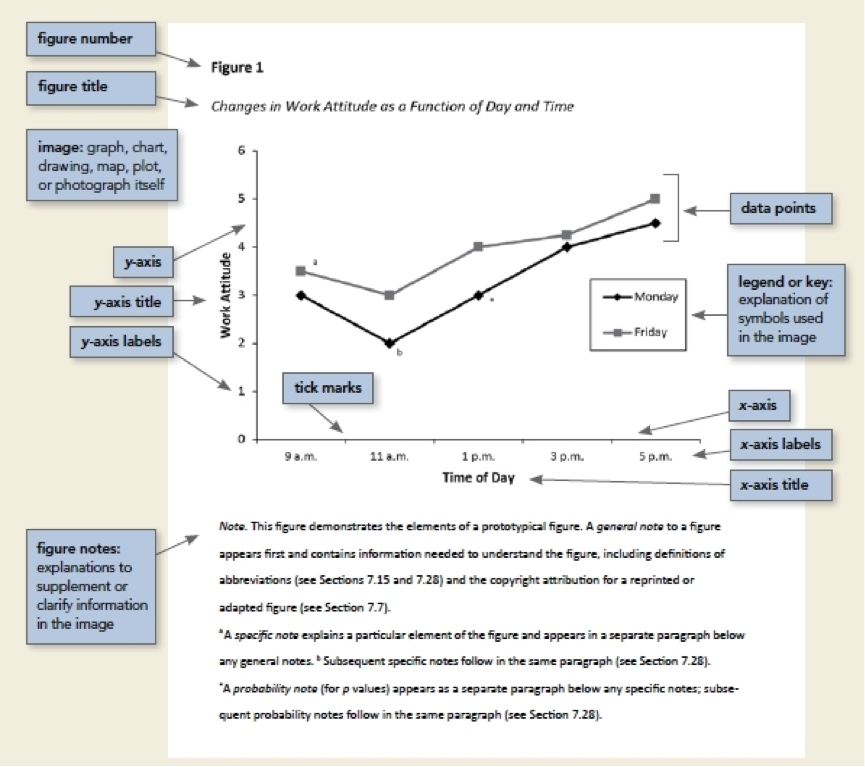
\includegraphics[width=0.7\textwidth]{images/figura.png}
      \caption{Ejemplo de figura externa representada como una imagen.}
      \label{fig:ejemplo_figura}
  \end{figure}
  
  \subsubsection{Consejos sobre figuras}
  Para diagramas, gráficas o ilustraciones técnicas, es preferible usar herramientas como `TikZ` o `PGFPlots` en lugar de imágenes externas.  
  Esto mantiene consistencia tipográfica, escalabilidad y edición directa desde el código fuente.
  
 
\clearpage 
 
\chapter*{Epílogo}
\phantomsection % punto de referencia para hipervínculos.
\addcontentsline{toc}{chapter}{Epílogo} % Agrega el epílogo al índice
\markboth{Epílogo}{Epílogo} % Define encabezado del epílogo

% Aquí comienza el contenido del epílogo
El epílogo es una parte final donde se resumen los puntos clave o se hace una reflexión sobre el contenido presentado en el libro. Puede incluir agradecimientos adicionales, comentarios sobre el proceso de escritura o ideas para futuros proyectos.

\section*{Reflexión Final}
% Aquí puede ir una reflexión más personal o general
Aquí va tu reflexión o conclusión final sobre el tema tratado en el libro.

\section*{Agradecimientos}
% Puedes agregar un agradecimiento en el epílogo
Quiero expresar mi agradecimiento a todas las personas que han contribuido a la realización de este libro y a quienes me han apoyado a lo largo de este proyecto.

% Aquí puedes continuar con más secciones o párrafos según lo necesites.
 
%=============================================================
% Material de extra
%=============================================================
 %=== Apendices
 
 \appendix
 \phantomsection
\begin{appendices}

%===========================================================
% Apendice A
%===========================================================

 \chapter{Apendices}
 \section{Apendice A}
 \label{sec:Apendice A}
 Este apéndice contiene información técnica adicional que complementa el capítulo de resultados.
 
 \subsection{Detalles técnicos del experimento}
 \subsubsection{Especificaciones del equipo}
 
 \begin{itemize}
   \item Modelo del sensor: XYZ-100
   \item Precisión: $\pm 0.01$ unidades
   \item Frecuencia de muestreo: 1 kHz
 \end{itemize}
 
 \subsubsection{Configuraciones del software}
 
 Las simulaciones fueron ejecutadas usando el entorno de desarrollo ABC en su versión 2.4.1.  
 El código fuente está disponible en el repositorio del proyecto.
 
 \subsubsection{Notas adicionales}
 
 Se realizaron pruebas preliminares para calibrar el sistema. Los resultados de estas pruebas no se incluyen en el cuerpo principal del documento por motivos de claridad.

%===========================================================
% Apendice B
%===========================================================

\section{Apendice B}
 
\end{appendices}




 
 
 %=== Glosarios (puedes simplemente comentar lo que no uses)
 
 \let\cleardoublepage\clearpage % No genera hoja al terminar impar
 \printglossary[type=acronym, title={Lista de abreviaciones}]
 \let\cleardoublepage\clearpage 
 \printglossary[type=symbols, title={Glosario de símbolos}]
 \let\cleardoublepage\clearpage 
 \printglossary[title={Glosario de términos}]
 \let\cleardoublepage\clearpage 
 \printglossary[type=constantes, title={Constantes físicas}]
 
 % Bibliografia
 %\nocite{*} % Forza a imprimir todas las entradas de la bibliografia 
 \let\cleardoublepage\clearpage 
 \printbibliography 
 
 \clearpage
 \chapter*{Colofón} % Evita numeración del capítulo
\phantomsection % Punto de anclaje para hipervínculos
\addcontentsline{toc}{chapter}{Colofón} % Lo agrega al índice

Este libro fue compuesto en \LaTeX, un sistema de composición tipográfica de alta calidad.

El diseño y la maquetación fueron realizados utilizando la clase de documento previamente definida en este proyecto.

La tipografía utilizada en el cuerpo del texto es \textit{Computer Modern}
La impresión y encuadernación fueron realizadas por [nombre de la imprenta o detalles de impresión].

\vfill

% Información centrada al pie de página
\begin{center}
  \small
  \textit{Este documento fue elaborado como parte del proyecto X.} \\
  \textit{Autor: Nombre del autor.} \\
  \textit{Fecha de finalización: Abril 2025.}
  
  \vspace{1em}

  \textcopyright~
  Año, Nombre del Autor.
\end{center}

 
 
\end{document}
